%%%%%%%%%%%%%%%%%%%%%%%%%%%%%%%%%%%%%%%%%%%%%%%%%%%%%%%%%%%%%%%%%%%%%%%%%%%%%%%%

\section{Maintenance}

%%%%%%%%%%%%%%%%%%%%%%%%%%%%%%%%%%%%%%%%%%%%%%%%%%%%%%%%%%%%%%%%%%%%%%%%%%%%%%%%

\begin{frame}[fragile]{EXPLAIN PLAN}

   TODO
   WIP

\begin{toile}
\toileurl{XXXX}
\end{toile}

\end{frame}

%%%%%%%%%%%%%%%%%%%%%%%%%%%%%%%%%%%%%%%%%%%%%%%%%%%%%%%%%%%%%%%%%%%%%%%%%%%%%%%%

\begin{frame}[fragile]{Tâches de maintenance de la base de données}

   La base de données nécessite des opérations de maintenance régulière pour assurer un service optimal.
   Les principales tâches de maintenance sont:
   \begin{itemize}
      \item Les sauvegardes régulières qui permettront de s'en sortir en cas d'accident grave
      \item Les opérations de VACUUM
      \item Les mises à jour des statistiques
      \item Les mises à jour des indexes
      \item La gestion des logs
   \end{itemize}

\begin{toile}
\toileurl{https://www.postgresql.org/docs/15/maintenance.html}
\end{toile}

\end{frame}

%%%%%%%%%%%%%%%%%%%%%%%%%%%%%%%%%%%%%%%%%%%%%%%%%%%%%%%%%%%%%%%%%%%%%%%%%%%%%%%%

\begin{frame}[fragile]{Les opérations de VACUUM}

   Les opérations de VACUUM sont lancées automatiquement par le démon \textsf{autovacuum}. Certains DBAs préfèrent gérer ce process eux-même à partir de tâches de type cron.
   Les raisons principales pour lancer un VACUUM régulier sont:

   \begin{itemize}
      \item récupérer l'espace disque occupé pour des lignes mises à jour ou supprimées
      \item mises à jour des statistiques utilisées par le planificateur de requêtes (query planner)
      \item mises à jour du flag de visibilité pour améliorer la performance des indexes only scan (chapitre Optimisation)
      \item protection contre la perte de données très anciennes causée par la rotation des identifiants de transaction ou de multi-transaction
   \end{itemize}

\begin{toile}
\toileurl{https://www.postgresql.org/docs/15/routine-vacuuming.html}
\end{toile}

\end{frame}

%%%%%%%%%%%%%%%%%%%%%%%%%%%%%%%%%%%%%%%%%%%%%%%%%%%%%%%%%%%%%%%%%%%%%%%%%%%%%%%%

\begin{frame}{Différents type de VACUUM}

   Il existe 2 types de VACUUM:
   \begin{itemize}
      \item le VACUUM standard
      \item le VACUUM FULL 
   \end{itemize}

\end{frame}

%%%%%%%%%%%%%%%%%%%%%%%%%%%%%%%%%%%%%%%%%%%%%%%%%%%%%%%%%%%%%%%%%%%%%%%%%%%%%%%%

\begin{frame}{VACUUM standard}

   \begin{itemize}
      \item Le VACUUM standard peut être lancé en parallèle des commandes SQL (\textbf{SELECT}, \textbf{UPDATE}, \textbf{INSERT} et \textbf{DELETE})
      \item la commande \textbf{ALTER TABLE} ne peut être exécutée sur une table en cours de traitement par le process
      \item le VACUUM génère des I/O très importantes qui diminuent les performances des autres sessions actives
      \item Il est possible de tempérer la charge I/O causée par le VACUUM par l'intermédiaire des paramètres: \textbf{vacuum\_cost\_*},
   \end{itemize}

\end{frame}

%%%%%%%%%%%%%%%%%%%%%%%%%%%%%%%%%%%%%%%%%%%%%%%%%%%%%%%%%%%%%%%%%%%%%%%%%%%%%%%%

\begin{frame}{Les paramètres \textbf{vacuum\_cost\_*}}

   Lors de l'exécution des commandes VACUUM et ANALYZE, le serveur garde une trace des coûts I/O engendrés par ces opérations. Lorsque l'accumulation de ces coûts atteint un seuil paramétrable, le process en cours de VACUUM est mis en sommeil pour une durée paramétrable et les coûts sont remis à 0.
   \begin{itemize}
      \item \textbf{vacuum\_cost\_delay}: durée de temps en millisecond pendant laquelle le process VACUUM sommeille
      \item \textbf{vacuum\_cost\_page\_hit}: coût associé au traitement d'une page dans les shared\_buffers (1)
      \item \textbf{vacuum\_cost\_page\_miss}: coût associé à une page en disque (2)
      \item \textbf{vacuum\_cost\_page\_dirty}: coût associé à une page modifiée (dirty page). Elle va nécessiter un flush vers le disque et de l'I/O (20)
      \item \textbf{vacuum\_cost\_limit}: seuil à partir duquel le process est mis en sommeil (200 par défaut)
   \end{itemize}

   Les valeurs par défaut sont adaptées.

\begin{toile}
\toileurl{https://www.postgresql.org/docs/15/runtime-config-resource.html\#RUNTIME-CONFIG-RESOURCE-VACUUM-COST}
\end{toile}
   
\end{frame}

%%%%%%%%%%%%%%%%%%%%%%%%%%%%%%%%%%%%%%%%%%%%%%%%%%%%%%%%%%%%%%%%%%%%%%%%%%%%%%%%

\begin{frame}{VACUUM FULL}

   \begin{itemize}
      \item Ce VACUUM récupère plus d'espace disque que le standard.
      \item Il est cependant plus lent
      \item Le VACUUM FULL posse un verrou de type \textbf{ACCESS EXCLUSIVE} sur la table en cours de traitement. Il empêche tout autre traitement d'accéder à la table.
      \item Il est recommandé de privilégier l'utilisation du VACUUM standard
   \end{itemize}

\end{frame}

%%%%%%%%%%%%%%%%%%%%%%%%%%%%%%%%%%%%%%%%%%%%%%%%%%%%%%%%%%%%%%%%%%%%%%%%%%%%%%%%

\begin{frame}{Récupération de l'espace disque}

   \begin{itemize}
      \item Le \textbf{DELETE} ou \textbf{UPDATE} ne supprime pas immédiatement les anciennes versions d'une ligne afin que les process ayant accès à la table ait leur version courante de la ligne jusqu'à la fin de la transaction.
      \item Lorsqu'une version devient obsolète et qu'elle n'est plus utilisée par une session, le VACUUM marque l'espace occupé par la ligne comme disponible pour les prochaines lignes.
      \item Cela permet d'éviter l'explosion de l'espace disque occupé par une table.
      \item L'espace disque n'est donc pas libéré: il devient disponible.
      \item Dans le cas où l'espace disponible se trouve en fin de page et qu'il est facile d'acquérir un verrou de type exclusif, l'espace disque est rendu à l'OS
   \end{itemize}

\end{frame}

%%%%%%%%%%%%%%%%%%%%%%%%%%%%%%%%%%%%%%%%%%%%%%%%%%%%%%%%%%%%%%%%%%%%%%%%%%%%%%%%

\begin{frame}{Récupération de l'espace disque}

   \begin{itemize}
      \item A l'inverse, VACUUM FULL réécrit entièrement la table de manière compacte sans espace vide. Cela réduit la taille occupée par la table mais prend beaucoup de temps.
      \item Durant le VACUUM FULL, l'espace disque de la table double car l'ancienne version est gardée jusqu'à la fin de l'opération
   \end{itemize}

\end{frame}

%%%%%%%%%%%%%%%%%%%%%%%%%%%%%%%%%%%%%%%%%%%%%%%%%%%%%%%%%%%%%%%%%%%%%%%%%%%%%%%%

\begin{frame}{Fréquence de passage du VACUUM}

   \begin{itemize}
      \item La bonne pratique est de lancer un VACUUM standard suffisamment fréquemment pour éviter de lancer le FULL
      \item Le démon autovacuum respecte cette philosophie et n'utilise pas le FULL
      \item L'objectif n'est pas de garder une taille minimale pour les tables
      \item L'objectif est de garder une taille des tables \textbf{stable}
      \item Pour appliquer le VACUUM sur une base de données entière, il est possible d'utiliser \textsf{vacuumdb}
   \end{itemize}

\end{frame}

%%%%%%%%%%%%%%%%%%%%%%%%%%%%%%%%%%%%%%%%%%%%%%%%%%%%%%%%%%%%%%%%%%%%%%%%%%%%%%%%

\begin{frame}{Cas des tables totalement supprimées}

   \begin{itemize}
      \item Lorsqu'une table est entièrement supprimée, la commande \textbf{TRUNCATE} peut être appliquée
      \item TRUNCATE libère automatiquement l'espace disque
      \item \textbf{Limitation:} le TRUNCATE ne respecte les principes du MVCC (vue locale des données pour chaque session)
   \end{itemize}

\end{frame}

%%%%%%%%%%%%%%%%%%%%%%%%%%%%%%%%%%%%%%%%%%%%%%%%%%%%%%%%%%%%%%%%%%%%%%%%%%%%%%%%

\begin{frame}{Cas des tables massivement mises à jour}

   \begin{itemize}
      \item Lorsqu'une table est massivement mise à jour ou supprimée, il peut être intéressant de lancer un VACUUM FULL
      \item Une alternative au VACUUM FULL est la commande \textbf{CLUSTER}
      \item Cette commande réécrit la table en disposant les lignes en suivant l'ordre de l'index d'une colonne
      \item Elle est décrite plus en détail dans la partie optimisation
   \end{itemize}

\end{frame}

%%%%%%%%%%%%%%%%%%%%%%%%%%%%%%%%%%%%%%%%%%%%%%%%%%%%%%%%%%%%%%%%%%%%%%%%%%%%%%%%

\begin{frame}{vacuumdb}

   \begin{itemize}
      \item VACUUM s'applique sur une table.
      \item Pour l'appliquer sur une base de données, il est possible d'utiliser \textbf{vacuumdb}
   \end{itemize}

\begin{toile}
\toileurl{https://www.postgresql.org/docs/15/app-vacuumdb.html}
\end{toile}

\end{frame}

%%%%%%%%%%%%%%%%%%%%%%%%%%%%%%%%%%%%%%%%%%%%%%%%%%%%%%%%%%%%%%%%%%%%%%%%%%%%%%%%

\begin{frame}{Mise à jour des statistiques du planificateur de requêtes}

   \begin{itemize}
      \item Le planificateur de requêtes s'appuie sur les statistiques collectées sur les tables
      \item La commande \textbf{ANALYZE} exécute la génération de statistiques sur une table
      \item L'ANALYZE est également une option de la commande VACUUM. De cette manière, les 2 opérations sont lancées en parallèle sur la table.
      \item L'ANALYZE est également une option du démon \textbf{autovacuum}
      \item Dans le cas où l'administrateur système sait que les mises à jour de la table n'affecte pas les statistiques, il est possible de gérer l'ANALYZE manuellement.
      \item \textbf{Les mises à jour dans les partitions de table ou les tables enfants ne provoquent d'ANALYZE automatique des tables parentes.}
      \item Pour cela, il est nécessaire de lancer l'ANALYZE manuellement sur les tables parentes.
   \end{itemize}

\begin{toile}
\toileurl{https://www.postgresql.org/docs/15/sql-vacuum.html}
\end{toile}

\end{frame}

%%%%%%%%%%%%%%%%%%%%%%%%%%%%%%%%%%%%%%%%%%%%%%%%%%%%%%%%%%%%%%%%%%%%%%%%%%%%%%%%

\begin{frame}{Cas des tables fréquemment mises à jour}

   \begin{itemize}
      \item En fonction de la répartition des valeurs de données dans une colonne, il peut être intéressant ou non de lancer la commande ANALYZE
      \item Pour des données ayant une plage de valeurs importante, l'ANALYZE est intéressant
      \item Dans le cas inverse, il n'est pas nécessaire dans le lancer
      \item L'ANALYZE peut être être restreint à une \textbf{colonne}. Particulièrement, celles impliquées dans les clauses WHERE avec une répartition de valeurs extrêmement irrégulière.
      \item En pratique, il s'avère plus efficace d'appliquer l'ANALYZE à la base de données
   \end{itemize}

\end{frame}

%%%%%%%%%%%%%%%%%%%%%%%%%%%%%%%%%%%%%%%%%%%%%%%%%%%%%%%%%%%%%%%%%%%%%%%%%%%%%%%%

\begin{frame}{Qualité des statistiques}

   Pour augmenter l'échantillonage de l'ANALYZE, il est possible d'utiliser 2 paramètres:
   \begin{itemize}
      \item \textbf{default\_statistic\_target}. Par défaut, 100. La base de données sera impactée
      \item \textbf{ALTER TABLE SET STATISTICS}. Seule la table sera impactée.
   \end{itemize}

\begin{toile}
\toileurl{https://www.postgresql.org/docs/15/runtime-config-query.html\#GUC-DEFAULT-STATISTICS-TARGET}
\end{toile}

\end{frame}

%%%%%%%%%%%%%%%%%%%%%%%%%%%%%%%%%%%%%%%%%%%%%%%%%%%%%%%%%%%%%%%%%%%%%%%%%%%%%%%%

\begin{frame}{Mise à jour du tableau de visibilité}

\begin{itemize}
   \item La table de visibilité de chaque page indique si une page de données est visible à toutes ltransactions actives.
   \item Si elle a été modifiée par une session et est en attente de flush vers le disque (dirty page), elle sera traitée par le VACUUM.
   \item Sinon elle ne sera pas traitée par le VACUUM.
   \item Le module \textbf{pg\_visibility} permet de visualiser les informations stockées dans la table de visibilité.
   \item La table de visibilité est utilisée pour les index-only scans pour éviter à l'index de rafraîchir les données qu'il embarque.
\end{itemize}

\begin{toile}
\toileurl{https://www.postgresql.org/docs/15/storage-vm.html}
\toileurl{https://www.postgresql.org/docs/15/pgvisibility.html}
\end{toile}
   
\end{frame}

%%%%%%%%%%%%%%%%%%%%%%%%%%%%%%%%%%%%%%%%%%%%%%%%%%%%%%%%%%%%%%%%%%%%%%%%%%%%%%%%

\begin{frame}{Prévention des erreurs causées par la rotation des identifiants de transaction}

\begin{itemize}
   \item Chaque transaction (XID) a un identifiant stocké sur un entier de 32 bits
   \item Cela autorise $2^{32}$ transactions
   \item Au bout de ce nombre de transaction, le compteur XID repasse à 0
   \item Les transactions qui étaient dans le passé se retrouvent dans le futur
   \item Pour prévenir ce type de situation, PostgreSQL utilise un identifiant spécial \textbf{FrozenTransactionId}
   \item Cet identifiant est antérieur à toute valeur de XID
   \item C'est le rôle du VACUUM de positionner cet identifiant de transaction sur la ligne
\end{itemize}

\end{frame}

%%%%%%%%%%%%%%%%%%%%%%%%%%%%%%%%%%%%%%%%%%%%%%%%%%%%%%%%%%%%%%%%%%%%%%%%%%%%%%%%

\begin{frame}{Rayon de $2^{31}$ pour chaque XID}

\begin{itemize}
   \item D'après ce qui a été dit précédemment chaque XID voit:
   \begin{itemize}
      \item Les $2^{31}$ transactions plus anciennes que lui
      \item et $2^{31}$ transactions futures
   \end{itemize}
   \item Une ligne ne sera jamais plus \textit{âgée} que $2^{31} = 2$ millions transactions
   \item A partir d'un certain âge paramétrable, son XID est gelé en FrozenTransactionId
\end{itemize}

\end{frame}

%%%%%%%%%%%%%%%%%%%%%%%%%%%%%%%%%%%%%%%%%%%%%%%%%%%%%%%%%%%%%%%%%%%%%%%%%%%%%%%%

\begin{frame}{VACUUM \textbf{agressif}}

\begin{itemize}
   \item le VACUUM s'appuie sur la table de visibilité pour savoir s'il est nécessaire de traiter la table et supprimer les versions obsolètes des lignes
   \item Il est cependant parfois nécessaire de geler les XID et MXID d'un certain âge
   \item Cette opération s'appelle le VACUUM \textbf{agressif}
\end{itemize}

\end{frame}

%%%%%%%%%%%%%%%%%%%%%%%%%%%%%%%%%%%%%%%%%%%%%%%%%%%%%%%%%%%%%%%%%%%%%%%%%%%%%%%%

\begin{frame}{Age d'une ligne - \textbf{vacuum\_freeze\_min\_age}}

\begin{itemize}
   \item \textbf{vacuum\_freeze\_min\_age} indique le nombre de transactions au-delà duquel VACUUM envisage de traiter une \textbf{ligne} de table pour geler son XID
   \item Une valeur trop basse de ce paramètre déclenche le gel \textsf{potentiellement inutile} d'une ligne avec le risque qu'elle soit dégelée en cas de modification
   \item Une valeur trop haute de ce paramètre augmente le nombre de transactions nécessaires avant que cette \textbf{ligne} de table puisse être traitée à nouveau par le VACUUM
   \item Valeur comprise entre 0 et $10^{9}$. Par défaut, $50*10^{6}$ transactions.
   \item Valeur automatiquement cappée à $\textbf{autovacuum\_freeze\_max\_age}/2$
\end{itemize}

\begin{toile}
\toileurl{https://www.postgresql.org/docs/15/runtime-config-client.html\#GUC-VACUUM-FREEZE-MIN-AGE}
\end{toile}

\end{frame}

%%%%%%%%%%%%%%%%%%%%%%%%%%%%%%%%%%%%%%%%%%%%%%%%%%%%%%%%%%%%%%%%%%%%%%%%%%%%%%%%

\begin{frame}{Age d'une table - \textbf{vacuum\_freeze\_table\_age}}

\begin{itemize}
   \item Le serveur applique un VACUUM \textbf{agressif} à la table lorsque \textbf{vacuum\_freeze\_table\_age} - \textbf{vacuum\_freeze\_min\_age} est positif
   \item Lorsque $\textbf{vacuum\_freeze\_table\_age} = 0$, un VACUUM agressif est systématiquement appliqué
   \item \textbf{pg\_class.relfrozenxid} est le niveau du XID en dessous duquel tous les XID de la table ont été gelés
\end{itemize}

\begin{toile}
\toileurl{https://www.postgresql.org/docs/15/catalog-pg-class.html}
\end{toile}

\end{frame}

%%%%%%%%%%%%%%%%%%%%%%%%%%%%%%%%%%%%%%%%%%%%%%%%%%%%%%%%%%%%%%%%%%%%%%%%%%%%%%%%

\begin{frame}{\textbf{autovacuum} et \textbf{vacuum\_freeze\_min\_age}}

\begin{itemize}
   \item la durée maximale qu'une table ne soit pas traitée par un VACUUM agressif est: $2^{31} - \textbf{vacuum\_freeze\_min\_age}$
   \item La valeur de \textbf{vacuum\_freeze\_min\_age} est stockée au passage du dernier VACUUM agressif
   \item L'\textbf{autovacuum} est déclenché lorsque $\textbf{autovacuum\_freeze\_max\_age} - \textbf{vacuum\_freeze\_min\_age}$ est positif.
   \item Pour empêcher la perte de données, il est déclenché même si \textbf{autovacuum\_freeze\_max\_age} n'est pas positionné
   \item Le gel des lignes opéré par le lancement de VACUUM est influencé par \textbf{vacuum\_freeze\_table\_age}
   \item La limite maximale posée par PostgreSQL est: $\textbf{vacuum\_freeze\_table\_age} = 0.95 * \textbf{autovacuum\_freeze\_max\_age}$
\end{itemize}

\end{frame}

%%%%%%%%%%%%%%%%%%%%%%%%%%%%%%%%%%%%%%%%%%%%%%%%%%%%%%%%%%%%%%%%%%%%%%%%%%%%%%%%

\begin{frame}{Paramètre \textbf{autovacuum\_freeze\_max\_age}}

\begin{itemize}
   \item Une valeur plus élevée de \textbf{vacuum\_freeze\_table\_age} est inutile (car le VACUUM agressif sera déclenché par \textbf{autovacuum\_freeze\_max\_age})
   \item Une valeur moins élevée de \textbf{vacuum\_freeze\_table\_age} déclenchera des VACUUM agressifs plus fréquents
   \item Le seul inconvénient d'augmenter \textbf{autovacuum\_freeze\_max\_age} entraîne un espace disque plus important occupé par les répertoires: 
      \begin{itemize}
         \item \textbf{pg\_xact}
         \item \textbf{pg\_commit\_ts}
      \end{itemize}
   \item Valeur par défaut: $200*10^{6}$ 
\end{itemize}

\begin{toile}
\toileurl{https://www.postgresql.org/docs/15/runtime-config-autovacuum.html\#GUC-AUTOVACUUM-FREEZE-MAX-AGE}
\end{toile}

\end{frame}

%%%%%%%%%%%%%%%%%%%%%%%%%%%%%%%%%%%%%%%%%%%%%%%%%%%%%%%%%%%%%%%%%%%%%%%%%%%%%%%%

\begin{frame}{Schéma récapitulatif}

\begin{figure}
\begin{center}
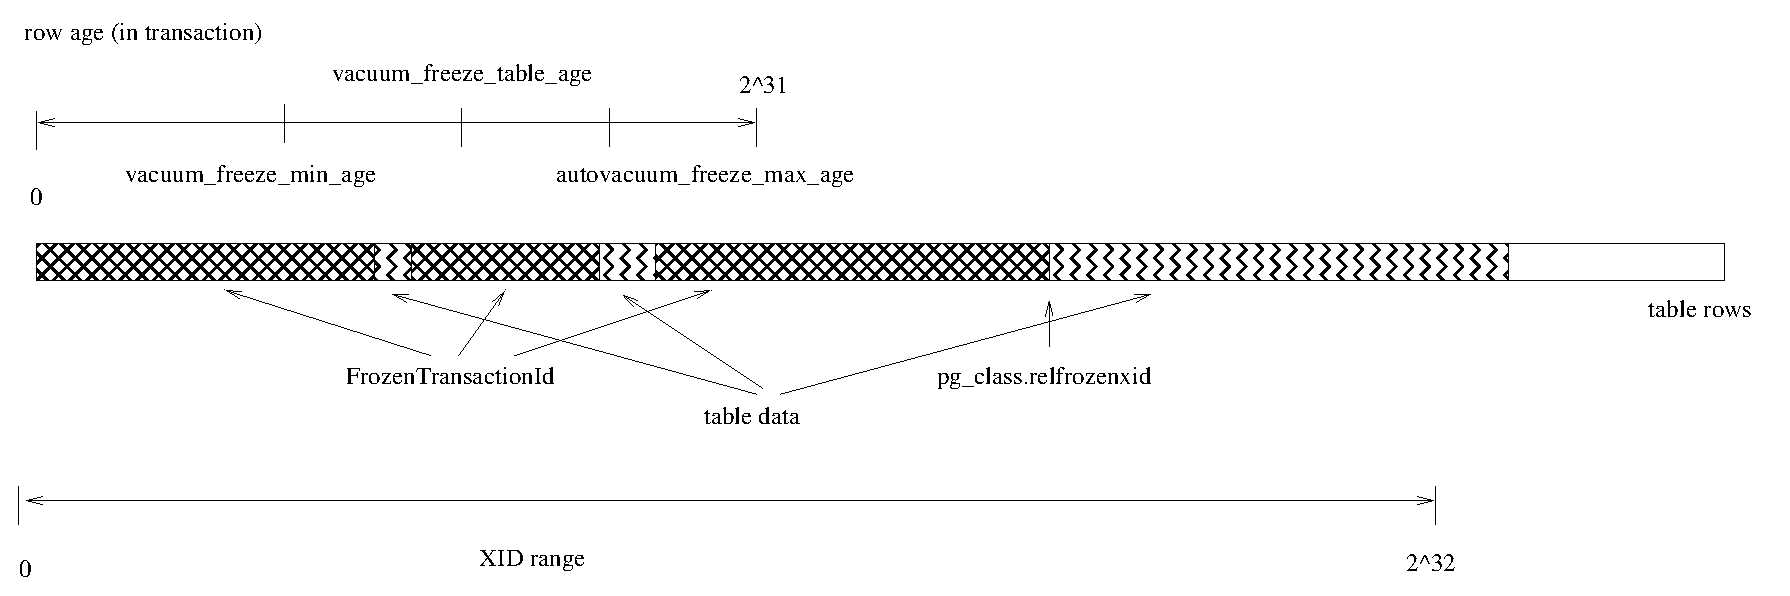
\includegraphics[angle=0, width=\textwidth]{images/xid_freeze.eps}
\end{center}
\end{figure}

\end{frame}

%%%%%%%%%%%%%%%%%%%%%%%%%%%%%%%%%%%%%%%%%%%%%%%%%%%%%%%%%%%%%%%%%%%%%%%%%%%%%%%%

\begin{frame}{Les répertoires \textbf{pg\_xact} et \textbf{pg\_commit\_ts}}

\begin{itemize}
   \item WIP
\end{itemize}

\end{frame}

%%%%%%%%%%%%%%%%%%%%%%%%%%%%%%%%%%%%%%%%%%%%%%%%%%%%%%%%%%%%%%%%%%%%%%%%%%%%%%%%

\begin{frame}[fragile]{Tests de vérification de la bonne santé de la base}

   TODO
   WIP

\begin{toile}
\toileurl{https://bucardo.org/check\_postgres/}
\end{toile}

\end{frame}

%%%%%%%%%%%%%%%%%%%%%%%%%%%%%%%%%%%%%%%%%%%%%%%%%%%%%%%%%%%%%%%%%%%%%%%%%%%%%%%%
